\chapter{Bound diffusion measurements}\label{ch04}
\label{ch:bound-diffusion}

Bound-state mobility - the ability of a macromolecule to diffuse while binding to its environment - was the key parameter in our simplified model of selective transport in Chapter~\ref{ch02}.  After many false starts, we designed an experimental system to investigate bound diffusion in biomaterials.  This hydrogel nuclear pore mimic, as described in Chapter~\ref{ch03}, is inspired by the nuclear pore but does not attempt to exactly reproduce selective nuclear transport.  Instead, it is designed to provide a method of measuring the effect of model parameters such as binding valency, tether length, and tether concentration on bound diffusion.

Diffusion of transport factors and inert proteins was measured within the Nup-filled hydrogels using two main methods: by quantifying the influx of these proteins into the hydrogels, and by measuring fluorescence recovery after photobleaching (FRAP) using hydrogels equilibrated with fluorescent proteins.  FRAP relies on the gradual redistribution of fluorophores after patterned photobleaching.   After a small portion of the hydrogel is bleached, the bleached spot gradually exchanges with the non-bleached fluorophores outside, and the average fluorescence intensity within the bleached spot recovers.  The recovery lifetime can be used to determine the fluorophore's diffusion constant, and the final recovered intensity as compared to the intensity outside the bleach spot can be used to determine the mobile fraction of fluorophore.  Many models of FRAP exist, including some that take binding into account \cite{sprague04, wu12, kang10, kang12}. We made use of several models of varying degrees of complexity.

We calculated bound diffusion constants for NTF2 in hydrogels containing FSFG concat-1 or FSFG concat-2 and found non-zero bound diffusion in both cases.  Both tether lengths led to bound diffusion that was consistent with that predicted by our tethered-diffusion model.

\section{Experimental parameters}

Our reaction-diffusion model of selectivity is controlled by a relatively small number of parameters.  Ideally, we would like to vary all of these experimentally in order to verify the model's predictions.  In reality, most are highly difficult to alter in a well-controlled way.  Of the model's parameters, the contour length $L_C$ of the tethered Nups is the simplest to control.  Varying this contour length will very the bound diffusion coefficient $D_B$ according to Eqn.~\ref{eq:dbound}.  This section discusses $L_C$ and the other experimental parameters used in our hydrogel nuclear pore mimics.

\subsection{Nup contour length and valency}

The most straightforward way to vary $D_B$ is to change the contour length of the Nups that are anchored into the hydrogel.  To that end, we compared hydrogels containing the constructs FSFG concat-1 and FSFG concat-2 (Sec.~\ref{sec:Nups}, Appendix~\ref{appx:sequences}).  These Nup fragments have $L_C = 50$ nm and 100 nm, respectively.  Given the parameters described below, the bound diffusion constant should increase by roughly 40\% from FSFG concat-1 to FSFG concat-2.

In addition to differing lengths, the FSFG concat-1 and concat-2 differ in their number of binding sites, with six and twelve respectively.  In order to control for the change in binding valency, we tested FSFG concat-2 hydrogels with the same molar concentration of FG repeats as the FSFG concat-1 gels as well as testing gels with the same molar concentration of Nups.

\subsection{Binding affinity of NTF2 and FSFG}
% ITC data is in book 1, a bit of book 2.  None of the fits were good.  Data shown here is taken from the runs on 6/18/14 and 6/23/14.  Fits aren't shown because we never really understood them.
Although bound diffusion is the key parameter from our reaction-diffusion model of selectivity, the kinetic parameters of off-rate $\koff$, on rate $\kon$, and dissociation constant $K_D = \koff/\kon$ are also important. These parameters are surprisingly difficult to measure, yielding values between 10 nM and 10 $\mu$M depending on the experimental conditions.  We estimated the dissociation constant for NTF2 and FSFG concat-1 using isothermal titration calorimetry (ITC).  The heat of injection was recorded as FSFG was titrated into a stock of NTF2.  While the resulting titration curves had low signal-to-noise and did not reach saturation, they clearly indicated binding (Fig.~\ref{fig:ITC-runs}).  Simple fits are likely inaccurate, given the high degree of multivalent binding, but may provide an order-of-magnitude estimate of the affinity.  Several ITC curves agree on a dissociation constant of $K_D \approx 200 \mu$M.  This is roughly compatible with the millimolar per-FSFG constant measured by the Rout lab with NMR and ITC \cite{hayama18}.  Similarly weak values were predicted through NMR, simulation, and stopped-flow anisotropy \cite{milles15}.

\begin{SCfigure}
\caption{Isothermal calorimetry titration curve: heat of injection vs. molar ratio of FSFG to NTF2. Fits are questionable but multiple runs suggest $K_D \approx 200\ \mu$M.\\}
\centering
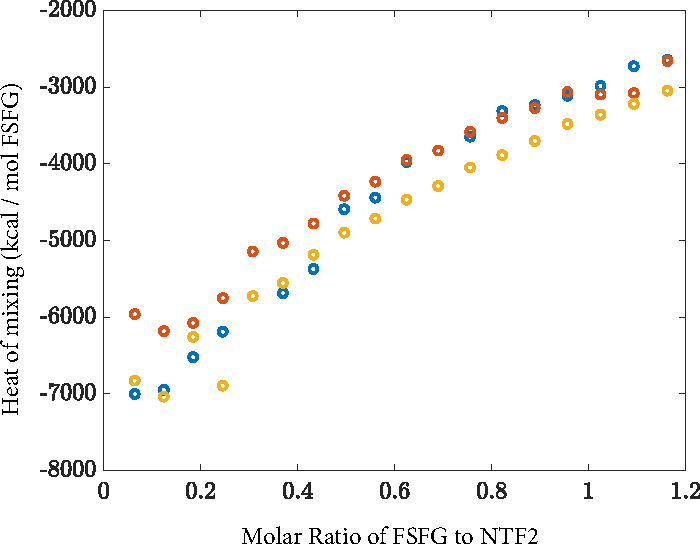
\includegraphics[width=0.6\textwidth]{figs/ch04/ITC_runs}
\label{fig:ITC-runs}
\end{SCfigure} 

Due to the twin difficulties of varying $K_D$ in a controlled way and accurately measuring its value, we did not attempt to experimentally alter this parameter.  Ideally, a transport factor - Nup pair with $K_D \approx 1 \mu$M would have been used to maximize selectivity.  For the purposes of determining the bound diffusion constant, the only value that is necessary to measure is the ratio $K_D/N_T$, which can be estimated using the partitioning of transport factors and inert proteins into the FSFG hydrogels (Sec.~\ref{sec:part-coeff}).  We investigated using the ubiquitin-associated (UBA) domain of the mRNA exporter Mex67 as a Nup-binding domain in GFP fusion proteins.  In principle, varying numbers of this small ($<$10 kDa) domain could be added to GFP to explore the effect of varying binding affinity and valency in transport factors.  The constructs GFP-UBA, GFP-UBAx2, and GFP-UBAx3 were created by Eric Verbeke, but did not express and/or bind well.

%Eric did most of the UBA cloning I think
% Expression tests in LKM book 5 pgs 146-9

\subsection{Quantifying concentration of tethered Nups}

Another potentially-tunable parameter of the bound-diffusion model is $N_T$, the total concentration of tethered Nups.  It is straightforward to control the Nup concentration in the hydrogel precursor solution by resuspending a known mass of lyophilized proteion.  Nup concentrations up to $\sim 50$ mg/mL can be resuspended.  However, it is much more difficult to determine how much protein was tethered to the hydrogel upon crosslinking. 

 BCA protein quantitation assays were used to place upper bounds on $N_T$.  Two methods were attempted: incubating the hydrogel itself in the working reagent, and soaking the hydrogel in a known volume of buffer and testing the concentration of FSFG released.  When applying the first method, the hydrogel was first soaked to remove excess precursor solution and thoroughly rinsed.  The gel was placed into a 96-well plate and buffer added until the appropriate sample volume was reached.  A standard BCA protocol was then followed.  Upon incubation with the working reagent, the hydrogels turned purple, as expected.  Standard absorption measurements and processing yielded an estimate of 0.5 mg/mL tethered FSFG-concat 1; this should be taken as an approximate value only.  The second method, that of soaking hydrogels and measuring the FSFG released, placed a similarly-low upper bound on tethered FSFG concentration.  Hydrogels made with 5 $\mu$L of precursor solution were soaked in 45 $\mu$L buffer to equilibrate.  The buffer was then measured to have a concentration of 1.0 mg/mL FSFG, implying a tethered FSFG concentration of $<1$ mg/mL.
% LKM book 5 pgs 119 and later

The concentration of Nups within the pore may reach 100 mg/mL, depending on how compact the disordered FG Nups are.  The low concentration of tethered Nups that we were able to achieve is therefore a major barrier to selectivity.  It is likely that the disordered nature of FSFG makes the labeled end less accessible to the hydrogel scaffold than would be the case for an ordered protein.  In an effort to overcome this limitation, we tested other linkers and conjugation methods.  We conjugated the FSFG-cys to PEG-diacrylate of varying lengths (700 Da and 10 kDa), to multi-armed PEG-diacrylate, and to maleimide-PEG-acrylate.  While labeling was verified using Ellman's reagent (Appendix~\ref{appx:bis-labeling}), there was no noticeable difference in transport factor partitioning into these hydrogels.
% maleimide-PEGDA LKM book 6 pgs 7-10
% multi-armed PEGDA LKM book 5 pg 151
% basic PEGDA conjugations throughout book 5

\subsection{Free diffusion constant}

The final tunable parameter from the binding-diffusion model is the diffusion constant of the transport factor when it is not bound to a Nup, the free diffusion constant $D_F$.  Decreasing $D_F$ is predicted to increase a material's selectivity while decreasing the absolute flux of transport factor (Figs.~\ref{fig:parameter-variations}, \ref{fig:parameter-variations-abs-flux}).  The free diffusion is predominantly determined by the protein's size and the viscosity of the solution, according to the Stokes-Einstein equation $D = k_BT/6\pi\eta R$, where $k_BT$ is the thermal energy, $\eta$ the solution viscosity, and $R$ the particle radius.  The solution viscosity could potentially be increased using a viscous additive such as glycerol; however, these attempts appeared to interfere with the binding of NTF2 and FSFG.

The diffusion of the non-binding 30 kDa protein mCherry was used as a proxy for the free diffusion of similarly-sized NTF2 within the FSFG hydrogels.

\section{Experimental procedures}

The nuclear pore mimics in this dataset were designed with the lessons of Chapter~\ref{ch03} in mind.  They consist of hydrogels with the largest average pore size and simplest geometry: a single microliter-scale droplet.  While this geometry does not allow for direct measurements of selectivity, the in-gel diffusion constants of both NTF2 and mCherry can be determined and bound diffusion calculated.  Two types of experiments were carried out: influx experiments, in which the entry of fluorescent proteins into the hydrogels was monitored, and FRAP experiments, in which a portion of an equilibrated hydrogel was bleached and the recovery observed.  Both experiments provide a measurement of the proteins' diffusion constants.  These experiments were performed at CU's BioFrontiers Advanced Light Microscopy Core Facility.  Thanks go to Joseph Dragavon for much assistance with the microscopy.

\subsection{Hydrogel preparation}

Detailed precursor solution recipes are given in Appendix~\ref{appx:precursor-recipes}.  For the dataset analyzed in this chapter, all nuclear pore mimic hydrogels were 6\% acrylamide and contained 2 mM LAP.  The precursor was made with potassium transport buffer (PTB) and contained either FSFG concat-1 bis or FSFG concat-2 bis.  Lyophilized FSFG-bis was resuspended in PTB, allowed to sit at room temperature for at least 20 minutes, and added to the precursor solution.  After the precursor solution was thoroughly mixed, it was degassed in a vacuum desiccator for 10 minutes and immediately pipetted into a disassembled 400-$\mu$m-thick PDMS gasket chamber (Sec.~\ref{sec:gel-geometries}).  Drops between 0.5 and 2 $\mu$L were carefully pipetted onto the plastic slide and the chamber assembled around the drops.  Typically, each chamber measured a few centimeters on a side and contained a control gel with no Nups as well as one or more Nup-filled gels.  The chamber was then illuminated as uniformly as possible with 365 nm light at approximately 200 mW/cm$^2$ with a ThorLabs M365 LP1 LED.  Condensation around the gels indicated that they had crosslinked.  The chamber was immediately rinsed with at least 100 $\mu$L of PTB, filled with fresh PTB, and sealed with a PDMS slab and clingwrap.  The gels were left to soak at 4$^\circ$C for at least 12 hours so that any remaining precursor solution and protein could leave the gel.

\subsection{Influx of transport factor and inert protein}
After soaking in buffer, the buffer solution was removed by pipette or wicking with a Kimwipe and a fluorescent reservoir solution added.  Aspirating the chamber was avoided if possible, as it sometimes disturbed the seal between the gel and the chamber.  The reservoir solution contained 20 $\mu$M each freshly-thawed NTF2-fluorescein (NTF2-F) and mCherry in PTB.  The chamber was resealed after adding the solution.  If no influx experiment was planned, the gels were then allowed to  equilibrate for 24 hours before FRAP was performed.

When influx experiments were run, they began as soon as possible after loading the reservoir solution.  Videos were recorded at 4x magnification on an Olympus IX-81 widefield microscope using FITC (excitation 464-500 nm / emission 516-556 nm) and TRITC (excitation 532-544 nm / emission 573-613 nm) filter cubes.  Exposure times were typically 30-100 ms with 3-8 dB gain.  Videos consisted of 120 frames at one frame per minute. Minimal photobleaching took place over the course of these experiments.  After the influx experiment, the chamber was usually stored for equilibration 4$^\circ$C, protected from light, and a FRAP experiment performed the following day.

Influx experiments on hydrogels containing FSFG show binding of NTF2-F to mCherry (Fig.~\ref{fig:influx-images}).  A bright wavefront  of NTF2-F slowly progresses into the gel, while mCherry remains largely excluded.  As expected, mCherry equilibrates more rapidly than does NTF2-F, due to the lack of binding.  Influx experiments were analyzed as described in Sec.~\ref{sec:influx-analysis}.

 % '/Volumes/houghgrp/Processed Images/2019-2-21_5/results.mat'
%'/Volumes/houghgrp/Microscopy/190220/190220_profiles_02.vsi’
%Cct2
%grnScale = [0;0.07];
%redScale = [0.0183566033417258;0.0502479591058213];
%Image_series_figures.m
\begin{figure}
\caption{Influx image series.  A hydrogel containing a nominal 5 mg/mL FSFG concat-2 was challenged with 20 $\mu$M NTF2-F and mCherry.  The hydrogel shows selective entry of NTF2-F and has largely equilibratd within 24 hours.}
\centering
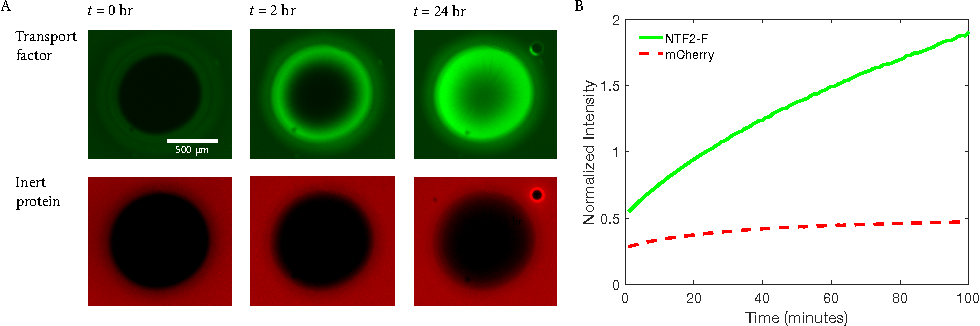
\includegraphics[width=0.9\textwidth]{figs/ch04/influx-images-clean.pdf}
\label{fig:influx-images}
\end{figure} 

\subsection{Fluorescence recovery after photobleaching}

FRAP is typically performed using a confocal microscope, but we were able to bleach the hydrogels using an Olympus IX-81 widefield microscope.  The widefield was preferable because the greater depth of field allowed for thicker hydrogel samples, which were easier to fabricate and manipulate.  As described above, the hydrogel was first allowed to equilibrate with 20 $\mu$M NTF2-F and mCherry in PTB.  A reference image was taken at 4x magnification in both fluorescence channels.  A circular region of the hydrogel around $300 \mu$m (?? check this) in radius was then photobleached by taking a five-second exposure at 40x magnification using a DAPI (excitation 352-402 nm / emission 417-477 nm) filter cube.  Following the bleach, the 4x objective was rapidly returned and a time series recorded.  Typical series consisted of 15-30 frames taken as rapidly as possible (5-10 s per frame), followed by 30-60 frames taken at a slower rate (1-2 minutes per frame).  Total experiment time was 1-4 hours.  Typical exposure times were 10 ms for NTF2-F and 40 ms for mCherry, both with a gain of 3 dB.

In order to increase throughput, up to three FRAP experiments were run concurrently by sequentially bleaching and then imaging several locations within a single chamber.  This led to a maximum delay time of approximately 35 s between the end of the bleach segment and the beginning of the time series.  Delay times were recorded and taken into account in the data processing. Figure~\ref{fig:frap-images} shows a representative series of images pre- and post-FRAP for both NTF2-F and mCherry.

Despite allowing 24 hours for equilibration, the fluorescence intensity across the hydrogel was not always uniform at the beginning of a FRAP experiment.  This could be due to slow diffusion into the hydrogels, or to inhomogeneous crosslinking.  The center of a hydrogel is more likely to be tightly crosslinked than the edges, as swelling is most inhibited at the center.  Gels which were too inhomogenous to display a clear bleach spot were discarded, but many nonuniform hydrogels were used in the final dataset, with the lack of equilibrium addressed in the data analysis (Sec.~\ref{sec:FRAP-analysis}).  Smaller hydrogels (0.5 $\mu$L of precursor solution) equilibrated more readily, at the cost of increasing the effect of fluorescent protein exchange with the reservoir, since the bleach spot then covered a significant fraction of the hydrogel.  This effect was also taken into account during data analysis.

% 2019-2-19, #21
%Cct1
%'/Volumes/houghgrp/Processed Images/2019-2-19_21/results.mat'
%[0.005;0.0222781719691768]
%Both scales
%Image_series_figures.m
\begin{figure} 
\caption{FRAP image series. NTF2-FITC (top, green) and mCherry (bottom, red) bleaching and recovery shown separately.  Hydrogel contained... }
\centering
\includegraphics[width=\textwidth]{figs/ch04/FRAP-images.pdf}
\label{fig:frap-images}
\end{figure} 

\section{Steady-state hydrogel properties}

Both the influx and FRAP experiments rely on steady-state properties of the hydrogel as well as time-dependent ones.  These properties include the partition coefficients of transport factors and inert proteins, as well as some dependent on the geometry of the hydrogel.

\subsection{Gel dimension estimates}
\label{sec:gel-dim}

% Small Hydrogel 19-2-6-21, grnScale [0.0;0.03], redScale [0.01;0.06], cropping rect 155.51 	0.51	1069.98 1023.98
% Large hydrogel 16	, '19-2-12_3'	'cct1'
\begin{SCfigure} 
\caption{Sample hydrogel masks with radius and center calculations.  (A) An equilibrated 0.5-$\mu$L hydrogel containing FSFG concat-1, immediately post-bleach. (B) The corresponding hydrogel mask (white), bleach spot mask (light gray), calculated gel diameter, and calculated gel center. (C)-(D) A 1-$\mu$L hydrogel, showing that the gel is not entirely within the field of view.}
\centering
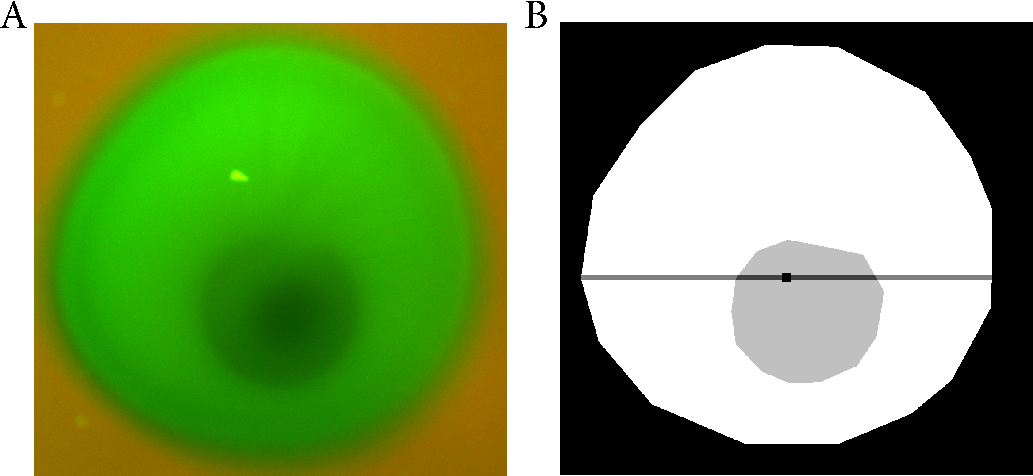
\includegraphics[width=0.5\textwidth]{figs/ch04/geometry.pdf}
\label{fig:masks}
\end{SCfigure} 

Although the hydrogels were not perfectly circular, all analysis treated them as circular or nearly so.  In total, the analysis made use of a gel's radius, center, perimeter, and area.  I began by manually defining two masks: one that covered the entire gel, and one that covered only the bleach spot (Fig.~\ref{fig:masks}).  The gel area was calculated by summing all of the pixels in the gel mask and, where necessary, making use of the 1.58 $\mu$m per pixel scale of the Olympus 4x objective.  The perimeter was calculated using Matlab's \texttt{bwperim} function, which takes a binary mask and returns a mask whose only nonzero entries are that mask's perimeter.  Summing over these pixels and scaling provides the gel perimeter.  It should be noted that in some cases the full area of the gel was not within the field of view.  In these cases, sometimes the partial area in the field of view was used as the area estimate, and sometimes I embedded the gel image in a larger frame and estimated the remaining area when drawing the mask.  Following sections indicate which method was used and the mathematical reasoning.  However, all perimeter calculations were performed with the estimated full area.

The hydrogel radius was estimated taking the diameter to be the widest row of the gel mask.  The widest row also set the $y$-coordinate of the gel center, with the $x$-coordinate calculated to be midway along the non-zero values for that row.  As seen in Fig.~\ref{fig:masks}, this is a quick and relatively crude method, but in almost all cases it works reasonably well.  An advantage of this method is that it works even for hydrogels which do not fit in the vertical field of view.

\subsection{Partition coefficients and fraction of time spent bound}
\label{sec:part-coeff}

% Hydrogel 19-2-6-21, grnScale [0.01;0.03], redScale [0.01;0.06], cropping rect 155.51 	0.51	1069.98 1023.98
\begin{SCfigure} 
\caption{Partitioning of NTF2 and mCherry into FSFG hydrogel.  (A) Partition coefficient $\gamma$ depends on whether the hydrogel excludes or binds protein. (B) Equilibrated FSFG concat-1 hydrogel (nominally 10 mg/mL) showing partitioning of $T_L = 20\ \mu$M each NTF2-FITC and mCherry.  Contrast adjusted for ease of viewing.\\}
\centering
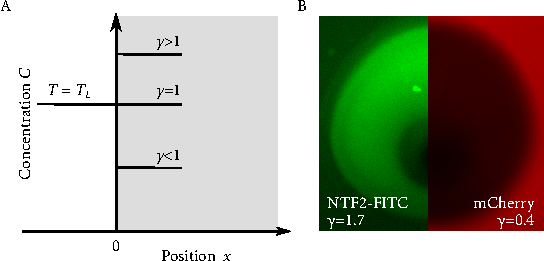
\includegraphics[width=0.6\textwidth]{figs/ch04/partition.pdf}
\label{fig:partition}
\end{SCfigure}

The concentration of NTF2 and mCherry in a flow chamber's reservoir can be directly controlled, but the partitioning of a protein into the hydrogel depends on the degree to which the presence of the gel sterically excludes the protein, as well as on binding interactions between the gel and protein.  When a transport-factor-sized inert protein is present to control for the steric effects, information about the transport factor's dissociation constant and fraction of time spent bound can be extracted from knowledge of the partition coefficient $\gamma$.  In particular, $p_B$, the fraction of time spent bound, is necessary in order to calculate the bound diffusion coefficient.

As shown in Fig.~\ref{fig:partition}A, the partition coefficient is the ratio of a protein's concentration in a well-equilibrated hydrogel to that in the surrounding reservoir.  This quantity is calculated by dividing the average intensity of the gel by that of the reservoir within the field of view (Fig.~\ref{fig:partition}B).  If the gel is not fully equilibrated, the partition coefficient can be estimated using a line scan through the reservoir and gel, though this will likely underestimate the true value.

When the system is in chemical equilibrium, the concentration of free transport factor ($T$), free Nup ($N$), and transport factor - Nup complex ($C$) is related to the dissociation constant $K_D$ by
%\begin{equation}
%K_D = \frac{TN}{C}
%\label{eq:chem-equil}
%\end{equation}
$K_D = NT/C \approx N_TT/C$ in the linear approximation $N \approx N_T$.   The total tethered Nup concentration, both free and bound, is the constant $N_T$.  The fraction of transport factors that are bound is then given by
\begin{equation}
p_B = \frac{C}{C+T} = \frac{C}{C+\frac{CK_D}{N_T}} = \frac{1}{1+\frac{K_D}{N_T}} %\approx 1 - \frac{K_D}{N_T}
\label{eq:bound-prob}
\end{equation} %where the final step applies if $K_D \ll N_T$, which might be the case but now I'm confused again.

To relate this expression to measureable quantities, write the protein concentrations within the hydrogel in terms of their partition coefficients. The concentration $c_0$ of the inert protein and the transport factor is equal in the reservoir.  If $\gamma_T$ is the partition coefficient of the transport factor and $\gamma_I$ that of the inert protein, then the transport factor concentrations can be expressed as
\begin{eqnarray}
T &=& \gamma_I c_0\\
C & =& T_T - T = \gamma_Tc_0 - \gamma_I c_0
\label{eq:gamma}
\end{eqnarray} 
The total transport factor concentration within the gel is $T_T = T + C$ and is a constant.
Therefore, within the gel, the chemical equilibrium condition can be expressed as
\begin{equation}
\frac{K_D}{N_T} = \frac{T}{C} = \frac{\gamma_I c_0}{\gamma_T c_0 - \gamma_I c_0} = \frac{\gamma_I}{\gamma_T - \gamma_I}
\label{eq:partition}
\end{equation}
Combining Eqns.~\ref{eq:bound-prob} and \ref{eq:partition}, the bound probability can be expressed in terms of the partition coefficients as
\begin{equation}
p_B= \frac{1}{1+\frac{K_D}{N_T}} = \frac{1}{1+\frac{\gamma_I}{\gamma_T - \gamma_I}} = 1 - \frac{\gamma_I}{\gamma_T}
\label{eq:bound-prob-final}
\end{equation}

\subsection{Bound-diffusion calculation}
\label{sec:db-calc}

Once the observed diffusion constants for NTF2 and mCherry have been calculated, along with the fraction of time spent bound $p_B$, the bound diffusion is given straightforwardly by the weighted average
\begin{equation}
D_\mathrm{obs, TF} = p_B D_B + (1-p_B) D_F
\label{eq:weighted-average}
\end{equation}
This result assumes Fickian diffusion.  In reality the diffusion will be slightly anomalous due to binding and the presence of the hydrogel.  However, the binding is highly transient and the hydrogel relatively permeable to proteins of the size of NTF2 and mCherry (Sec.~\ref{sec:pore-size}).

Taking the free diffusion coefficient of the transport factor to be approximately equal to the observed diffusion of the inert protein ($D_F = D_\mathrm{obs,I})$, the bound diffusion coefficient of the transport factor is
\begin{equation}
D_B = \frac{D_\mathrm{obs, TF}-(1-p_B) D_\mathrm{obs,I}}{p_B}
\label{eq:d-bound}
\end{equation}

Note that neither the dissociation constant or the total Nup concentration need to be measured independently in order to calculate the bound diffusion constant.

\section{Influx analysis}
\label{sec:influx-analysis}

%2/20/19 #2 , also 2-21-19 #5 first image, grn scale [0.0038; 0.023], red [0.00; 0.0381], crop rect [3.915100000000000e+02,1.755100000000000e+02,8.259800000000000e+02,7.979800000000000e+02]
\begin{figure}
\caption{Intensity profiles and total accumulation within hydrogel as determined from influx time series.  (A) Image of an FSFG concat-2 hydrogel with a nominal Nup concentration of 10 mg/mL. Reservoir contains 20 $\mu$M NTF2-F and mCherry in PTB. Reservoir mask is shown (red polygon) as well as accumulation area and rectangle over which the profile averaging was performed. (B) Normalized intensity profiles as calculated using the box in (A).  (C) Normalized average intensity within hydrogel.}
\centering
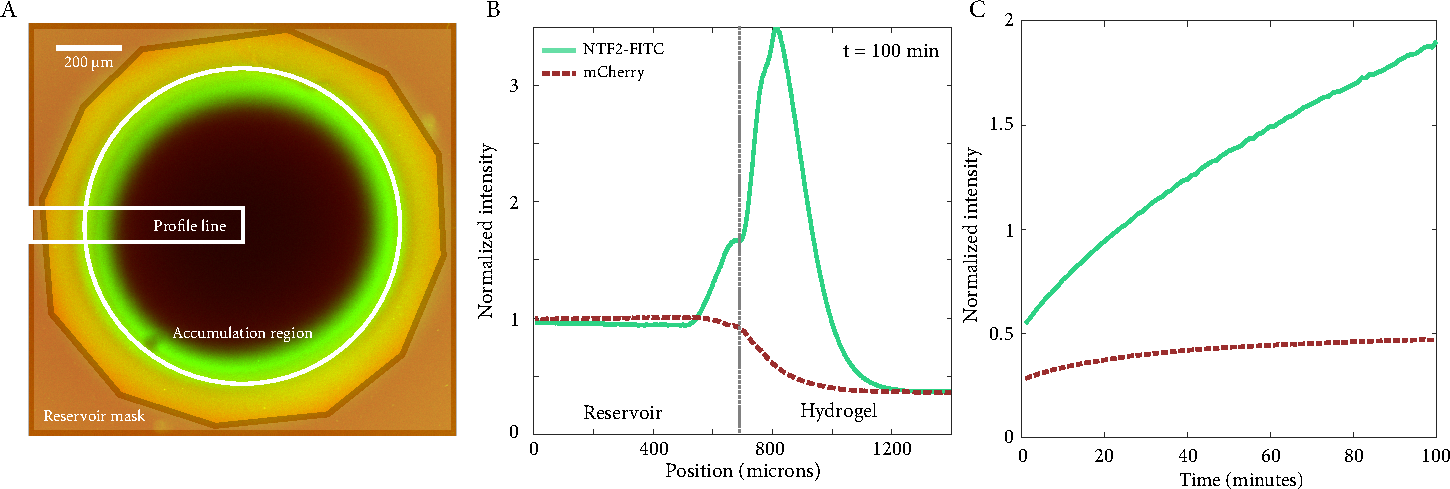
\includegraphics[width=\textwidth]{figs/ch04/influx-plots.pdf}
\label{fig:influx-plots}
\end{figure}

After recording a time series of fluorescent protein influx into a hydrogel, diffusion constants can be estimated using either a plot of the intensity profile across the gel or a plot of total accumulation within the gel.  Figure~\ref{fig:influx-plots} shows an example of each plot.  The intensity within the gel is normalized to the average intensity of the reservoir, as calculated using the mask shown in Fig~\ref{fig:influx-plots}A.  Therefore, each profile trace begins at $I=1$ within the reservoir and either dips or rises to the partition coefficient value within the gel.  As the gels are not equilibrated, much of the gel interior shows only background fluorescence.  Likewise, the average intensity within the hydrogel trends towards the partition coefficient but does not reach it on the time scale of an average experiment.

Analysis of the accumulation and profile curves used the diffusion-equation solutions described by Mortensen, Okkels, and Bruus \cite{mortensen06}.  This method assumes that the edge of  a nearly-circular two-dimensional region is held at a fixed concentration while the interior equilibrates (Fig.~\ref{fig:mortensen}.  Such boundary conditions correspond to an infinite fluorophore reservoir.  Given that our reservoirs are 10-20 times larger than the hydrogel volume, this is a reasonable assumption.  In a slight modification, we allow for an arbitrary partition coefficient $\gamma$ by taking the fixed boundary concentration $c_0$ to be $\gamma T_0$, where $T_0$ is the fluorescent protein intensity in the reservoir.  The assumption of near-circularity is also a good one.

\begin{SCfigure}
\caption{Geometry used to solve diffusion equation in \cite{mortensen06}.  The reservoir concentration $c_0$ fixed the concentration at the edge of the region $\Omega$.  The concentration $c(\mathbf{r},t)$ is determined within $\Omega$ as a function of position and time.}
\centering
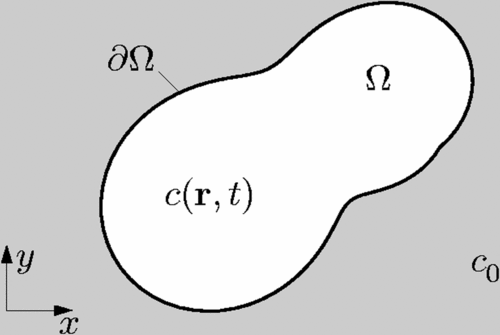
\includegraphics[width=0.4\textwidth]{figs/ch04/mortensen}
\label{fig:mortensen}
\end{SCfigure}

The two most troublesome restrictions of the Mortensen equations are Fickian diffusion and the homogeneity of the hydrogel.  As discussed in Sec.~\ref{sec:fickian}, the presence of the hydrogel meshwork and binding make diffusion within the hydrogels slightly anomalous.  Additionally, despite the improvements to the fabrication protocol, the hydrogels likely contain some degree of nonuniformity in their density, with the centers most likely being slightly denser than the edges due to differential swelling.  The effects of swelling and non-uniform thickness are greatest at the gel edge.  Unfortunately, the points at the edge of the gel and earliest in the experiment are the most important to the following fits.  As a result, the diffusion constants extracted using the profile and accumulation plots are not reliable.  The analysis is presented below nonetheless, as a similar approach was taken in analyzing the FRAP experiments.

\subsection{Profile analysis}
% figure  '180209_FSFG-gel_2.vsi'
\label{sec:profile-analysis}

Mortensen \textit{et al} first define a characteristic timescale for equilibration $\tau = (\mathcal{A}/\mathcal{P})^2 (\pi/4D)$ where $\mathcal{A}$ and $\mathcal{P}$ are the area and perimeter, respectively, of $\Omega$.  For a circle $\mathcal{A}/\mathcal{P} = a/2$, but this ratio was numerically calculated for the hydrogels (Sec.~\ref{sec:gel-dim}).  For times $t \ll \tau$, the concentration profile as a function of the distance $r$ from the gel center can be approximated as 
\begin{equation}
c(r,t) = c_0 \,\mathrm{erfc}\left(\frac{r}{\sqrt{4Dt}}\right)
\label{eq:approx-profile}
\end{equation}
where $D$ is the diffusion constant.

%% erfc position at fixed time '180525_FSFGPEGDA700_03.vsi'
%% t is close to beginning but not right at beginning

\begin{figure}
\caption{Fits to Eqn.~\ref{eq:approx-profile} near the beginning of the influx experiment for (A) mCherry and (B) NTF2-Alexa488 intensity profiles.  Hydrogel nominally contains 10 mg/mL FSFG-PEGDA 700 kDa.  The entire intensity profile is shown in the top panel with the portion used for fitting highlighted in red.  Approximate locations of the gel edge, background fluoresence level, and partition coefficient are also shown.}
\centering
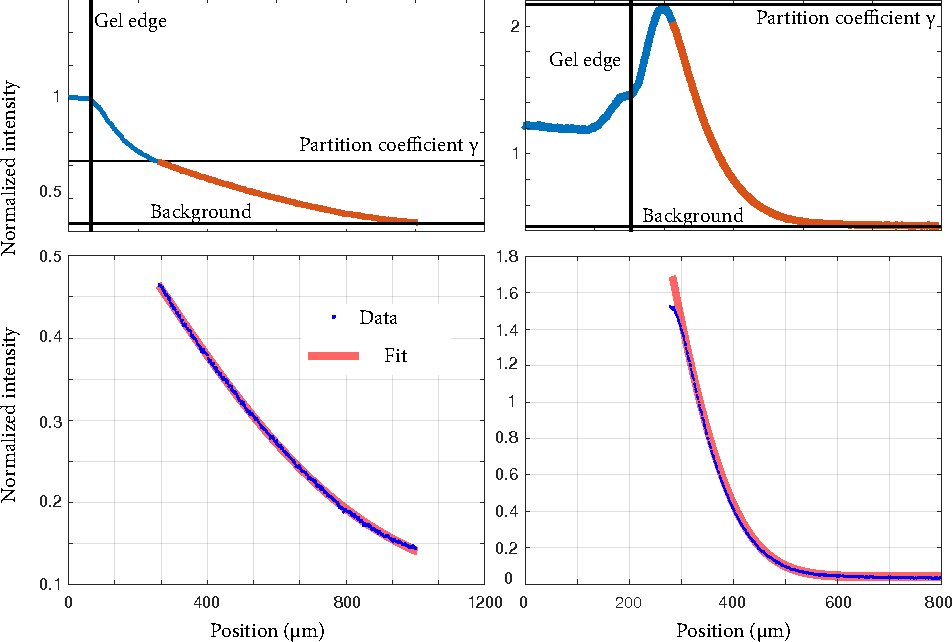
\includegraphics[width=0.9\textwidth]{figs/ch04/erfc-position.pdf}
\label{fig:erfc-position}
\end{figure} 

\begin{SCfigure}
\caption{Fits to Eqn.~\ref{eq:approx-profile} at a fixed point near the gel edge for (A) mCherry and (B) NTF2-Alexa488 intensity profiles.  The short-time approximation likely only holds for times $t \lesssim 20$ minutes. Hydrogel nominally contains 10 mg/mL FSFG-PEGDA 700 kDa.\\}
\centering
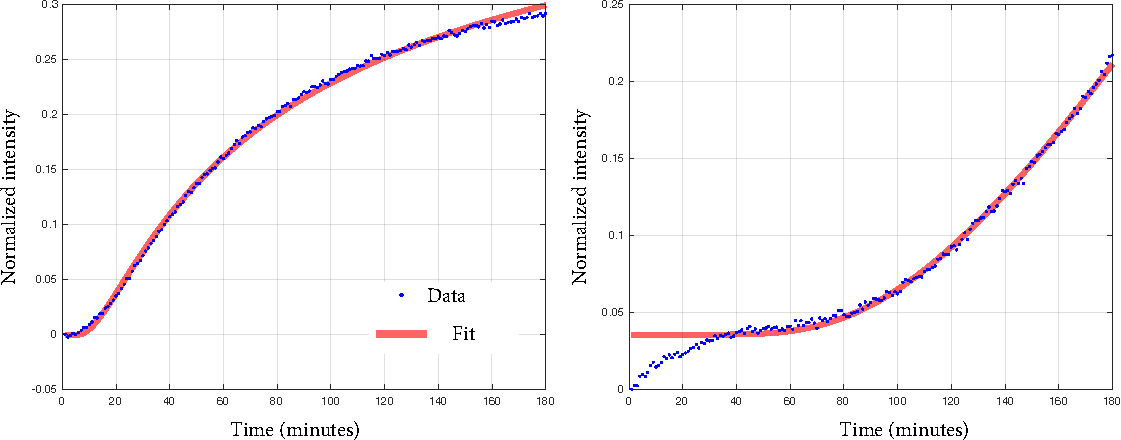
\includegraphics[width=0.7\textwidth]{figs/ch04/erfc-time.pdf}
\label{fig:erfc-time}
\end{SCfigure} 

The typical duration of an influx experiment was approximately $\tau$, making the short-time approximation questionable throughout most of the time series.  We attempted to fit the intensity profile (Fig.~\ref{fig:erfc-position}) and obtained fits with fairly low error but with unreliable fit parameters.  In addition to the issues of timescale, it was often difficult to determine where the gel edge was located, as well as the partition coefficient.  Given these problems, it is not surprising that fits at successive timepoints yielded incompatible values of diffusion constant for both mCherry and NTF2.  A similar problem prevented the use of diffusion constants obtained from intensity fits at a fixed position over time (Fig.~\ref{fig:erfc-time}).

A more exact solution for $c(r,t)$ can be written if the gel is assumed to be circular.  Mortensen \textit{et al} quantify the error introduced by small deviations from circularity and find it to be small.  Assuming a circular gel, the concentration profile at an arbitrary time $t$ is given by
\begin{equation}
\frac{c(r,t)}{c_0} = 1 - 2\sum_{n=0}^\infty \frac{J_0(\alpha_n r)}{\alpha_n a J_1(\alpha_n a)}\exp(-\alpha_n D t)
\label{eq:full-profile}
\end{equation}
where $a$ is the gel radius and $\alpha_n a$ is the $n$th zero of the Bessel function of the first kind $J_0$.

I fit the intensity profiles to Eqn.~\ref{eq:full-profile} using different numbers of terms $N$.  For the mCherry curves, the resulting fit parameters tended to converge as $N$ increased, and the RMSE stabilized.  However, neither was true for the NTF2 curves.  Increasing values of $N$ led to steadily decreasing values of diffusion constant.  This may be due to the effect of binding on NTF2 diffusion.

\subsection{Accumulation analysis}

The total accumulation within the hydrogel can be modeled by integrating the concentration profile over the entire gel.  When this is done, the averaged intensity within the hydrogel $N(t)$ is found to be
\begin{equation}
\frac{N(t)}{N_0} = 1-\sum_{n=0}^\infty \frac{4}{(\alpha_na)^2}\exp\left(-\frac{(\alpha_na)^2\pi t}{16\tau}\right)
\label{eq:full-accumulation}
\end{equation} where$N_0$ is the equilibrium value, here equal to the partition coefficient $\gamma$ once the intensity has been normalized to that of the reservoir.

\begin{SCfigure}
\caption{Accumulation fits to Eqn.~\ref{eq:full-accumulation} for (A) mCherry and (B) NTF2-Alexa488.  Hydrogel nominally contains 10 mg/mL FSFG-PEGDA 700 kDa.\\}
\centering
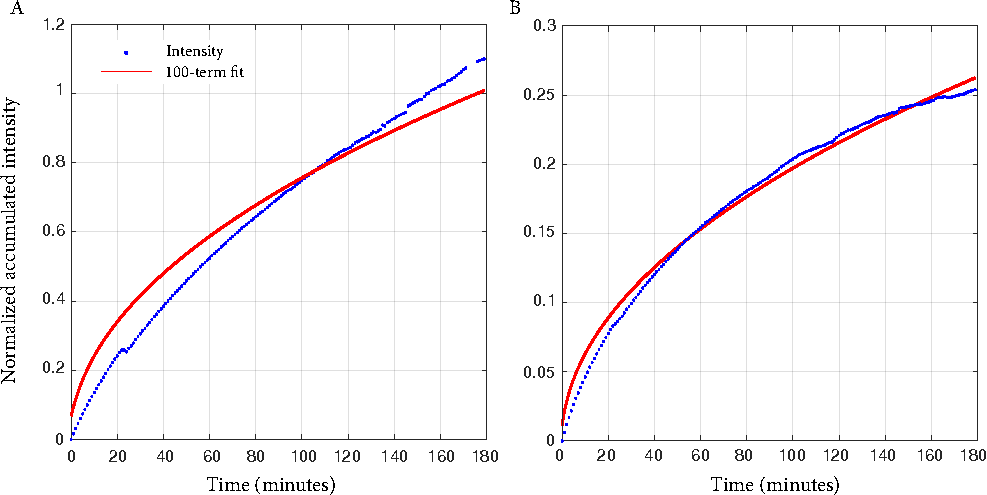
\includegraphics[width=0.7\textwidth]{figs/ch04/accumulation.pdf}
\label{fig:acc}
\end{SCfigure} 

% figure ''180516-FSFGbis_2.vsi'' fit to 100 terms, made with processing-4 script, results 11-12-18.mat

Fits to the first 100 terms of Eqn.~\ref{eq:full-accumulation} are shown in Fig.~\ref{fig:acc} for mCherry and NTF2.  These fits had systematic error, likely for the same reasons as the profile fits.

While the profile and accumulation data do contain information on the diffusion constants of NTF2 and mCherry, I was unable to reliably extract that information using the influx experiments.  The model presented above is a remarkably good match to the experimental setup except for the presence of binding and the unpredictable gel-edge effects.  The FRAP experiments overcome the problem of edge effects by making use of equilibrated regions deep within the hydrogel.

\section{FRAP analysis}
\label{sec:FRAP-analysis}

\subsection{Accounting for photobleaching}
\label{sec:photobleaching}
Small but noticeable amounts of photobleaching occur over the course of the FRAP experiment.  In order to correct for photobleaching, the intensity of the bleached spot must be normalized to that of the entire gel, including the bleached region.  The normalized intensity used to fit the recovery curves is given by
\begin{equation}
N(t) = \frac{c_b(t)}{c_g(t)}
\end{equation} where the average intensity of the bleach spot is $c_b(t) = C_b(t)/A_b$. The total intensity within the bleach spot is $C_b(t)$ and $A_b$ is the area of the spot as shown in Fig.~\ref{fig:masks}.  The average intensity of the entire gel $c_g(t)$ is defined similarly.  Using this normalization removes the effects of photobleaching, as verified by simulating recovery data with various photobleaching rates.

\subsection{No-exchange solution to diffusion equation}
\label{sec:no-exchange}

The simplest realistic model of fluorescence recovery assumes that the hydrogel is perfectly uniform and equlibrated, that the presence of the gel is unimportant, and that there is no exchange of fluorescent proteins between the hydrogel and the reservoir during the experiment.  Upon making those assumptions, the recovery curve can be fit using a sum of two Bessel functions as described in \cite{yang18,sprague04}.  The model used in \cite{sprague04} distinguishes between binding affinity regimes; NTF2-FSFG binding is sufficiently transient that it falls into the effective diffusion regime, allowing standard diffusion equations to be used without modification to calculate an effective diffusion constant as described in Sec.~\ref{sec:db-calc}.  The solution to fluorescence recovery with effective diffusion is given by
\begin{equation}
N(t) = A\exp(-\tau_D/2t)\left(\mathrm{I}_0(\tau_D/2t)+\mathrm{I}_1(\tau_D/2t)\right)+C
\end{equation} where the diffusion lifetime $\tau_D$ is related to the diffusion constant by $D = w^2/\tau_D$ if $w$ is the bleach spot radius.  

The amplitude $A$ and offset $C$ are related to the bleach depth (given by $C$) and final recovered value (given by $A+C$).  Typical bleach depths were 5-10\% of the initial intensity and tended to be smaller for mCherry than for NTF2.  In principle, the final recovered value reflects the immobile fraction of fluorophore.  If there is an immobile fraction, the bleached region will not recover to its intial value.  Given the weak binding between NTF2 and FSFG, we do not expect an appreciable immobile fraction of either NTF2 or mCherry.  For the most part, the hydrogels appear to recover to their initial value.  A few do not, for reasons that are unclear even after accounting for photobleaching.

The no-exchange model fits well to the larger hydrogels and those that are well-equilibrated.  Many of the large gels, however, were not fully equlibrated even after a 24 hour incubation with the reservoir solution.  The concentration within these gels will change over the course of the experiment as they continue to equilibrate.  Smaller hydrogels were quicker to uniformly equlibrate; however, these gels are small enough that exchange of fluorescent proteins with the reservoir is important over the timescale of FRAP recovery.  Both of these problems can be accounted for using a more thorough solution to the diffusion equation.

\subsection{Fourier transform solution to diffusion equation}
%Carslaw 2nd ed. pg 377, sec. 14.13(6)

To account for exchange of fluorescent proteins with the reservoir, as well as for incomplete equilibration, some of the assumptions of the previous section must be relaxed.  In particular, the assumption of radial symmetry must be abandoned.  In order to incorporate angular as well as radial dependence, the solution must be written as a sum over Bessel function and cosine modes.  While such a solution is cumbersome, it allows for an accurate description of the concentration throughout the hydrogel immediately post-bleach.  Additionally, the boundary condition can be defined so as to allow exchange between the hydrogel and reservoir.

This analysis begins by numerically calculating the two-dimensional polar Fourier transform of the initial concentration distribution within the gel, decomposing it into a finite number of modes weighted by their contribution to the image.  These mode coefficients are then used to create the equation to which the experimentally-measured recovery curve is fit.  The fit parameters include the observed diffusion coefficients for NTF2 and mCherry, allowing the bound diffusion constant to be determined as described in Sec.~\ref{sec:db-calc}.

Scripts to perform the following calculations are available at \url{https://github.com/LauraMaguire/image-processing}.

\subsubsection{Analytic series solution}

The problem is that of diffusion in a circular region of radius $a$, centered at the origin, whose boundary is held at a fixed concentration.  The region $r<a$ has an arbitary intial concentration distribution $f(r,\theta)$ which consists of the first post-bleach image (Fig.~\ref{fig:carslaw-geo}).  To find the concentration $c(r,\theta,t)$ for $r<a$, we used the Green's function integrals described in \cite{h.s.carslaw59}, as heat transfer obeys the same differential equation as diffusion of particles.  Green's functions describe a system's response to an instantaneous point source.  An initial distribution can be built by integrating the Green's function over the region of interest.  The correct Green's function must be identified for a particular geometry and set of boundary conditions, but a formal solution is straightforward to write once they have been obtained.

\begin{SCfigure}
\caption{Geometry for diffusion-equation solution Eqn.~\ref{eq:full-series}.  A circle of radius $a$ is centered at the origin.  The boundary $r=a$ is held at concentration $c=0$ and the interior has initial concentration profile $f(r,\theta)$.}
\centering
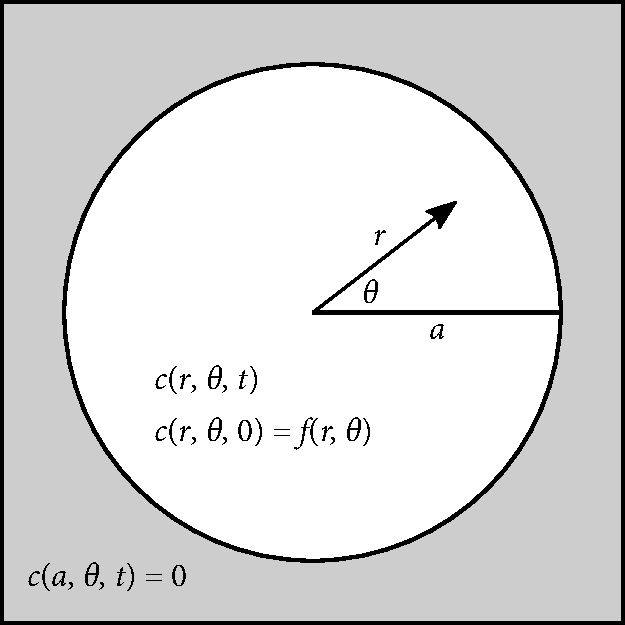
\includegraphics[width=0.35\textwidth]{figs/ch04/carslaw-geometry}
\label{fig:carslaw-geo}
\end{SCfigure} 

As this solution is two-dimensional, two sums must be taken over the basis functions.  Bessel functions $J_\nu$ of the first kind and integer order $\nu$ are the radial basis, and cosines are the angular basis.  The time dependence is carried by decaying exponentials whose time constant is related to the diffusion coefficient $D$ as well as to the zeros of the Bessel functions.  The terms are summed over the Bessel orders as well as over the zeros of each Bessel function.  For our situation, the full solution to the diffusion equation within the hydrogel is given by \cite{h.s.carlslaw59}

\begin{equation}
\begin{split}
c(r,\theta,t) =& \sum_{\nu=-\infty}^{\infty} \sum_{\alpha = 0}^\infty   \frac{\exp\left(-D\alpha^2t\right)J_\nu\left(\alpha r\right)}{\left(J'_\nu(\alpha a)\right)^2} \times \\ 
&b_{\nu,\alpha} \int_0^{2\pi} \int_0^a \cos\left(\nu(\theta-\theta')\right) J_\nu(\alpha r') f(r',\theta') r' dr' d\theta' \label{eq:full-series}
\end{split}
\end{equation}
where, as in the previous section, $\alpha a$ are the zeros of $J_\nu$, and $b_{\nu,\alpha}$ are normalization constants defined in Sec.~\ref{sec:calcCoeffs}.  Note that the sums run over all positive and negative integer Bessel orders and over all zeros of each Bessel function.  

This solution applies to a circle whose boundary is held at $c=0$, so it must be shifted by an offset in order to match the experimental concentration at the boundary.  Note that the relevant boundary concentration is just within the hydrogel, not the concentration of the reservoir.  The reservoir is assumed to be infinite, in order to maintain the hydrogel edge at its equilibrium concentration, but the concentration of the reservoir itself is irrelevant.

The integral above is difficult to use as written because it contains both primed and unprimed coordinates in the angular term, $\cos\left(\nu(\theta -\theta')\right)$.  The unprimed coordinate can be removed from the integral using the identity $$\cos(\phi_1-\phi_2) = \cos\phi_1\cos\phi_2 + \sin\phi_1\sin\phi_2$$ The mode coefficients $C_{\nu,\alpha}$ and $S_{\nu,\alpha}$ can then be defined as
\begin{equation}
c(r,\theta,t) = \sum_{\nu=-\infty}^{\infty} \sum_{\alpha = 0}^\infty   \frac{\exp\left(-D\alpha^2t\right)J_\nu\left(\alpha r\right)}{\left(J'_\nu (\alpha a)\right)^2} \left(C_{\nu,\alpha}\cos(\nu\theta) + S_{\nu,\alpha} \sin(\nu\theta)\right)
\label{eq:c-s-series}
\end{equation}
with 
\begin{eqnarray}
C_{n,\alpha} & = &b_{\nu,\alpha} \int_0^{2\pi} \int_0^a \cos\left(\nu\theta'\right) J_\nu(\alpha r')f(r',\theta') r' dr' d\theta' \label{eq:cos-defn}\\
S_{n,\alpha} & = & b_{\nu,\alpha}\int_0^{2\pi} \int_0^a \sin\left(\nu\theta'\right) J_\nu(\alpha r') f(r',\theta') r' dr' d\theta' \label{eq:sin-defn}
\end{eqnarray}
The problem is reduced to determining the mode coefficients by evaluating the integrals.

\subsubsection{Calculating mode coefficients}
\label{sec:calcCoeffs}

Before mode coefficients can be calculated using Eqns.~\ref{eq:cos-defn} and \ref{eq:sin-defn}, the normalization constants $b_{\nu,\alpha}$ must be determined.  To find an expression for them, begin with Eqn.~\ref{eq:c-s-series} at $t=0$, when $c(r,\theta,0) = f(r,\theta)$.
\begin{equation}
f(r,\theta)= \sum_{\nu=-\infty}^{\infty} \sum_{\alpha = 0}^\infty   \frac{J_\nu\left(\alpha r\right)}{\left(J'_\nu (\alpha a)\right)^2} \left(C_{\nu,\alpha}\cos(\nu\theta) + S_{\nu,\alpha} \sin(\nu\theta)\right)
\label{eq:c-s-series-t-0}
\end{equation}
This expression for $f(r,\theta)$ can be substituted into Eqns.~\ref{eq:cos-defn} and \ref{eq:sin-defn}.  Using the cosine coefficients as an example,
\begin{eqnarray*}
C_{n,\alpha} & = &b_{\nu,\alpha} \int_0^{2\pi} \int_0^a \cos\left(\nu\theta'\right) J_\nu(\alpha r') \times\\
& &\left[\sum_{\mu=-\infty}^{\infty} \sum_{\beta = 0}^\infty   \frac{J_\mu\left(\beta r'\right)}{\left(J'_\mu (\beta a)\right)^2} \left(C_{\mu,\beta}\cos(\mu\theta') + S_{\mu,\beta} \sin(\mu\theta')\right)\right] r' dr' d\theta'\\
C_{n,\alpha} & = &b_{\nu,\alpha} \sum_{\mu=-\infty}^{\infty} \sum_{\beta = 0}^\infty\int_0^{2\pi} \int_0^a \cos\left(\nu\theta'\right)  \frac{ J_\nu(\alpha r')   J_\mu\left(\beta r'\right)}{\left(J'_\mu (\beta a)\right)^2} \times\\
& & \left(C_{\mu,\beta}\cos(\mu\theta') + S_{\mu,\beta} \sin(\mu\theta')\right) r' dr' d\theta'\\
C_{n,\alpha} & = &b_{\nu,\alpha} \int_0^{2\pi} \int_0^a  \frac{ J_\nu^2(\alpha r')}{\left(J'_\nu (\alpha a)\right)^2} \left(C_{\nu,\alpha}\cos^2(\nu\theta') + S_{\nu,\alpha}\cos\left(\nu\theta'\right)\sin(\nu\theta')\right) r' dr' d\theta'
\end{eqnarray*}
The integral and sum have been switched and the orthogonality of the basis functions used to collapse the sums.  The integral of the $S_{\nu,\alpha}$ term vanishes, as it is an odd function ($\cos\left(\nu\theta'\right)\sin(\nu\theta')$) integrated over all $\theta'$.  Similarly, the $C_{\nu,\alpha}$ term drops from the sine coefficient integral.  The remaining term gives
\begin{eqnarray*}
C_{n,\alpha} & = &b_{\nu,\alpha} \int_0^{2\pi} \int_0^a  \frac{ J_\nu^2(\alpha r')}{\left(J'_\nu (\alpha a)\right)^2} C_{\nu,\alpha}\cos^2(\nu\theta') r' dr' d\theta'
\end{eqnarray*} or finally
\begin{equation}
\frac{1}{b_{\nu,\alpha}}  =  \int_0^{2\pi} \int_0^a  \frac{ J_\nu^2(\alpha r')\cos^2(\nu\theta') }{\left(J'_\nu (\alpha a)\right)^2} r' dr' d\theta' \label{eq:bna-theory}
\end{equation}

So long as the integral is truly over the entire circle $r<a$, this constant is the same for both $C_{\nu,\alpha}$ and $S_{\nu,\alpha}$.  In that case, Eqn.~\ref{eq:bna-theory} gives $b_{\nu,\alpha} = 2/\pi a^2$ for every mode.

However, in many cases, it is not possible to numerically integrate over the entire gel, as seen in Fig.~\ref{fig:masks}D.  All numerical integrals are instead over the gel mask, which encompasses as much of the gel as fits into the field of view.  The value of this mask is one within the gel and zero outside, so it serves to define the limits of numerical integration.  Denoting the area covered by this mask as $\Omega$, the normalization constants for $C_{\nu,\alpha}$ and $S_{\nu,\alpha}$, respectively, are
\begin{eqnarray}
1/b_{\nu,\alpha}^C  &= & \int_\Omega \frac{ J_\nu^2(\alpha r')\cos^2(\nu\theta') }{\left(J'_\nu (\alpha a)\right)^2} r' dr' d\theta' \label{eq:bna-c} \\
1/b_{\nu,\alpha}^S  &=  &\int_\Omega \frac{ J_\nu^2(\alpha r')\sin^2(\nu\theta') }{\left(J'_\nu (\alpha a)\right)^2} r' dr' d\theta' \label{eq:bna-s}
\end{eqnarray}

Likewise, the numerical integrals in Eqns.~\ref{eq:cos-defn} and \ref{eq:sin-defn} are more precisely written 
\begin{eqnarray}
C_{n,\alpha} & = &b_{\nu,\alpha}^C \int_\Omega \cos\left(\nu\theta'\right) J_\nu(\alpha r')f(r',\theta') r' dr' d\theta' \label{eq:cos-defn2}\\
S_{n,\alpha} & = & b_{\nu,\alpha}^S\int_\Omega \sin\left(\nu\theta'\right) J_\nu(\alpha r') f(r',\theta') r' dr' d\theta' \label{eq:sin-defn2}
\end{eqnarray}

The degree to which the resulting coefficients deviate from the ideal case of a perfect circle can be roughly quantified by the ratio $b_{\nu,\alpha} /(2/\pi a^2) = \pi a^2 b_{\nu,\alpha} /2$. For small hydrogels, which entirely fit into the field of view, these values range from 1.01 to 1.03, signifying deviations of up to 3\%.  Large hydrogels whose top and bottom were cut from the field of view had deviations of up to 10\%.  However, using Eqns.~\ref{eq:bna-c} and \ref{eq:bna-c} instead of the uniform mode weighting $b_{\nu,\alpha} = 2/\pi a^2$ should compensate for the irregular area of integration.

For every hydrogel, Bessel order $\nu$, and Bessel zero $\alpha$, mode coefficients were calculated numerically.  The polar coordinates $(r,\theta)$ were converted to Cartesian $(x,y)$ and a sum taken over all the pixels of the initial post-bleach image $f(x,y)$, using the hydrogel mask to set the limits.  The center of the coordinate system was set at the center of the gel and the value of the gel radius $a$ calculated as described in Sec.~\ref{sec:gel-dim}. Before the sum was calculated, the average intensity of the equilibrated portions of the hydrogel was subtracted from the entire image, effectively setting the equilibrium concentration at $c=0$ as required by the series solution.

The sum was scaled using the area represented by each pixel (using the scale 1.58 $\mu$m/pixel) and normalized using the weighting constants $b_{\nu,\alpha}$.  The final values of $C_{\nu,\alpha}$ and $S_{\nu,\alpha}$ were stored in two arrays for use in constructing the equation to which the experimental data was fit.

%\texttt{C(nu,alpha) = scale\^{}2*sum(sum( bC(nu,alpha)*mask*cos(atan2(nu*y/x))\\*J\_nu(sqrt(x\^{}2+y\^{}2))*image}

\subsubsection{Reconstruction of initial image}

To verify the mode coefficients, I reconstructed the initial post-bleach image from which they were calculated.  The image was reconstructed by numerically integrating Eqn.~\ref{eq:c-s-series-t-0} using a similar method to that discussed in the previous section.  The area outside the gel mask was not reconstructed.  Figure~\ref{fig:initDist} shows the resulting reconstructions as the number of terms in the series increases.  The relative magnitudes of those terms are plotted in Fig.~\ref{fig:arrays}.  The reconstruction is adequate for our purposes by the time $N_\nu = 20$ and $N_\alpha = 20$, i.e. twenty Bessel orders and twenty zeros are used.  Note that the Bessel orders are given by $\nu = -10,-9,...0...8,9$.  A coefficient array of this size allowed a dataset of 43 hydrogels to be entirely processed and fit in approximately 24 hours on a desktop computer; larger coefficient arrays would require the use of a computing cluster.

% #16 in dataset, '19-2-12_3', avg. gel intensity set to zero before calculating coefficients, green channel reconstruction
\begin{figure}
\caption{Reconstruction of initial concentration distribution. Reservoir is masked and not included.  (A) Heatmap of original image with average equilibrated gel intensity set to zero. (B) Reconstruction using two Bessel orders ($N_\nu = 2$) and two zeros ($N_\alpha = 2$) in each order. (C-E) Reconstructions with $N_\nu = N_\alpha = 4$, 10, and 20.}
\centering
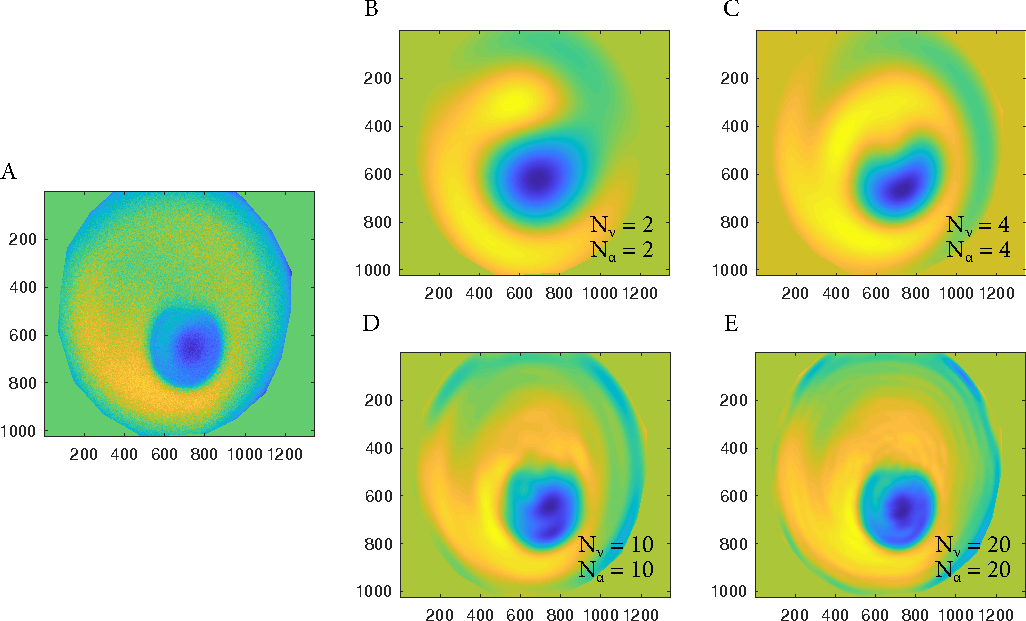
\includegraphics[width=0.9\textwidth]{figs/ch04/reconstruction-16_2_4_10_20.pdf}
\label{fig:initDist}
\end{figure} 

% #16 in dataset, '19-2-12_3', avg. gel intensity set to zero before calculating coefficients, green channel reconstruction
\begin{SCfigure}
\caption{Heatmap of cosine and sine mode coefficients $C_{\nu,\alpha}$ and $S_{\nu,\alpha}$ for the reconstruction shown in Fig.~\ref{fig:initDist}E. Values are shown for each Bessel order $\nu$ and each zero $\alpha$. \\}
\centering
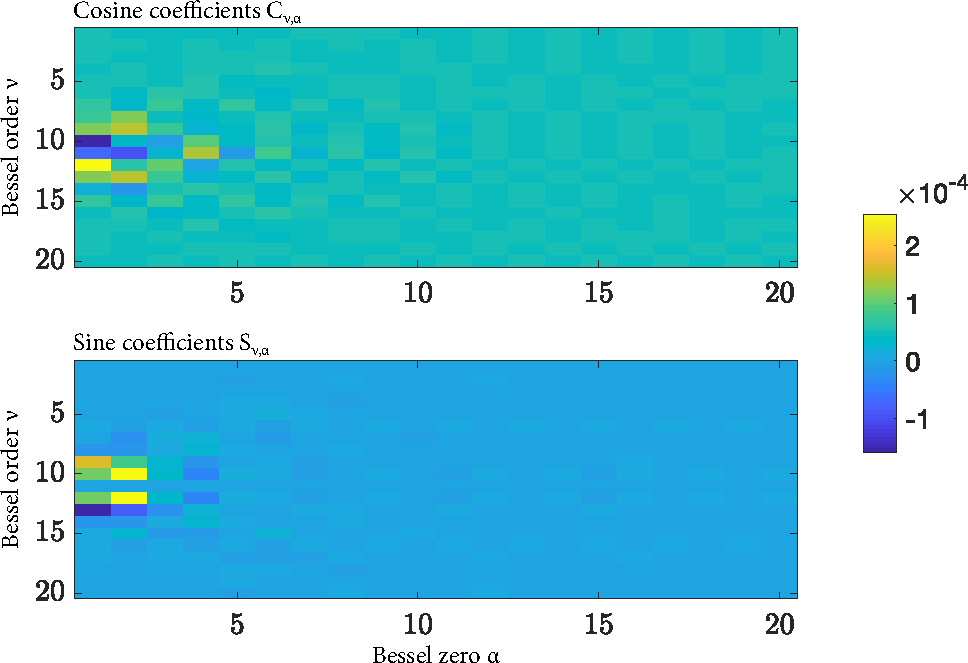
\includegraphics[width=0.7\textwidth]{figs/ch04/rec_16_cos_sin_array_20_terms.pdf}
\label{fig:arrays}
\end{SCfigure} 

\subsubsection{Fitting recovery curves}

Once the mode coefficients had been calculated, a fit string was constructed using the full series equation Eqn.~\ref{eq:c-s-series} and fed into the Matlab curve fitter.  Careful thought was required to ensure that the model was treated in the same way as the experimental data.

To begin, the mode coefficients were used to predict the average intensity of the bleach spot at each time point.  Since the time dependence in each term is only in a decaying exponential, the average value of the bleach spot could be determined by integrating over the bleach spot:
\begin{equation}
\bar{c}_\mathrm{bleach}(D,t) = \frac{1}{A_B}\sum_{\nu=-\infty}^{\infty} \sum_{\alpha = 0}^\infty   \exp\left(-D\alpha^2t\right)\int_{\Omega_B}\frac{J_\nu\left(\alpha r\right)}{\left(J'_\nu (\alpha a)\right)^2} \left(C_{\nu,\alpha}\cos(\nu\theta) + S_{\nu,\alpha} \sin(\nu\theta)\right) dA
\label{eq:c-s-series}
\end{equation}
where $\Omega_B$ is the region defined by the bleach-spot mask and $A_B$ its total area.  The Bessel function derivative $J'_\nu$ was computed using the identity
\begin{equation*}
J'_\nu(x) = \frac{1}{2}\left(J_{\nu-1}(x) - J_{\nu+1}(x)\right)
\end{equation*}

The average intensity of the entire gel, including the bleach spot, was determined in the same way, using the hydrogel mask instead of the bleach-spot mask.  Both results were formatted as strings of sums, containing numerical values wherever possible as well as the diffusion constant parameter $D$ (units of $\mu$m$^2$/s)  and the time variable $t$, measured in seconds.

Once these strings were created, the equilibrium concentration value $c_0$ was added back to both of them, and their ratio was taken, in order to mimic the data processing in Sec.~\ref{sec:photobleaching}.  Mathematically, this gave a normalized string of
\begin{equation}
f(D,t) = \frac{\bar{c}_\mathrm{bleach}(D,t)+c_0}{\bar{c}_\mathrm{gel}(D,t)+c_0}
\end{equation}

At this point, I checked the normalization by simulating data using the value of $D$ calculated from the no-exchange analysis in Sec.~\ref{sec:no-exchange}.  Often the simulated data matched the experiment to within 10\%, but further fit parameters were needed in order to fit the data well.  Ultimately, the function to which the data were fit was
\begin{equation}
g(c_1,c_2,D,t) = c_1f(D,t) + c_2
\end{equation}
where $c_1$ and $c_2$ reflect the bleach depth and final recovered concentration similarly to $A$ and $C$ in Sec.~\ref{sec:no-exchange}.  Their values are less important than that of the diffusion constant $D$.

Fits such as those shown in Fig.~\ref{fig:series-fits} were typical results.  Values for $c_1$ and $c_2$ were of order unity, except for a few fits that were clearly incorrect and were omitted from the final dataset.

% #'s 5 and 7 in the dataset
\begin{figure}
\caption{Fits using the series expansion Eqn.~\ref{eq:full-series}. (A) NTF2-F and mCherry recovery curves for a no-nup hydrogel.  (B) NTF2-F and mCherry recovery curves for a hydrogel nominally containing 10 mg/mL FSFG concat-1.}
\centering
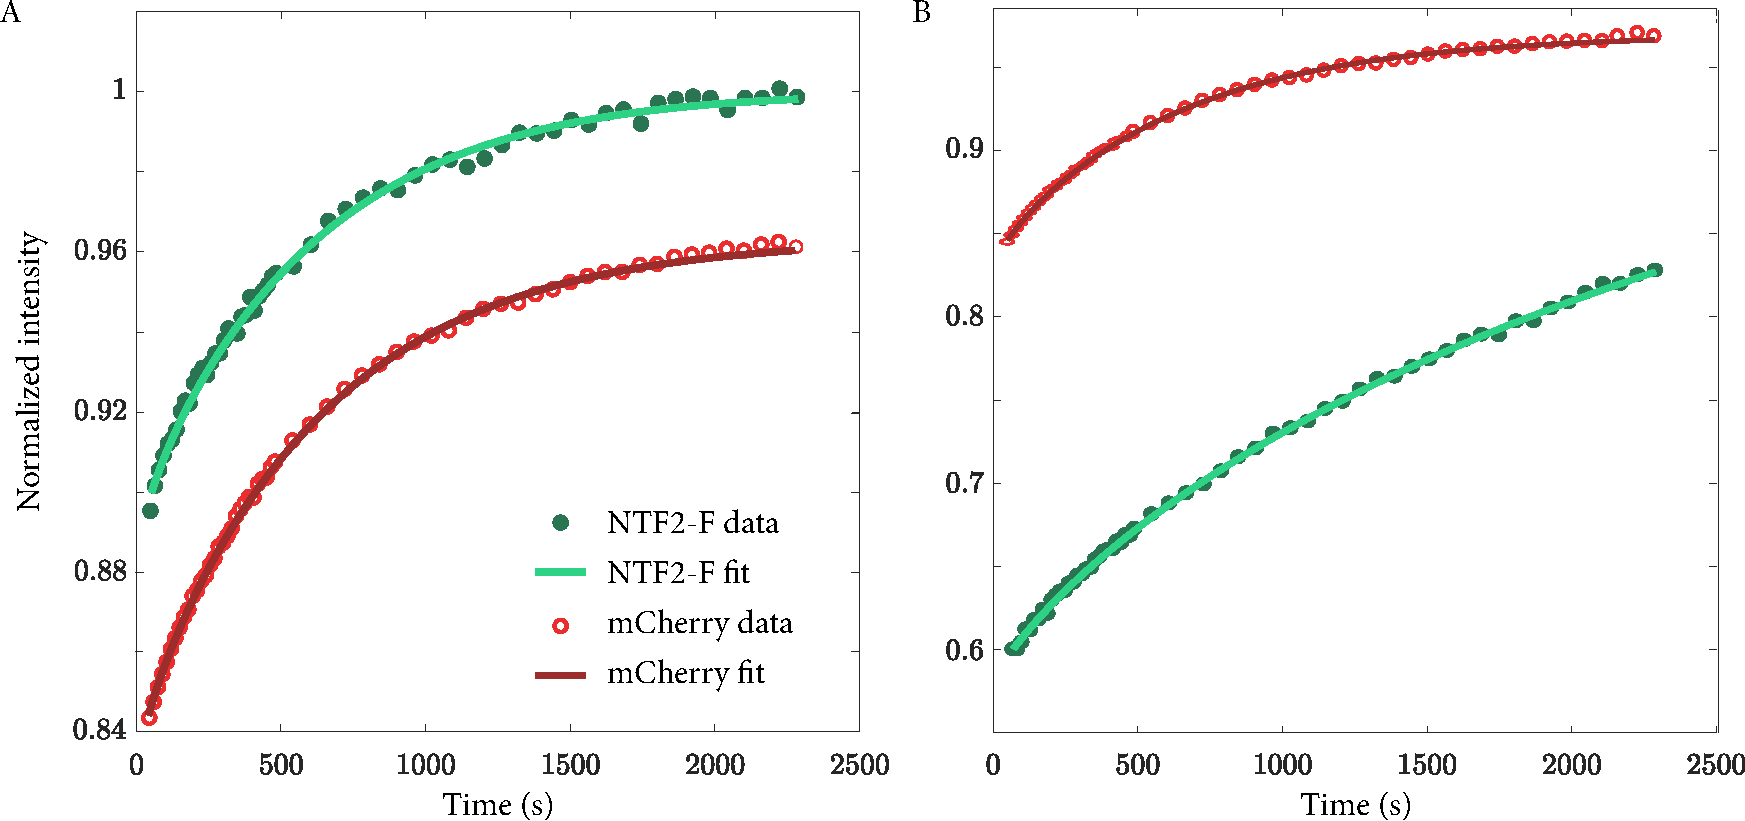
\includegraphics[width=0.9\textwidth]{figs/ch04/series-fits.pdf}
\label{fig:series-fits}
\end{figure} 

\section{Results}

In all, FRAP analysis was performed on 36 hydrogels: 15 no-nup gels, 12 nominally containing 10 mg/mL FSFG concat-1, and 7 containing FSFG concat-2 nominally at 20 mg/mL. % Of the FSFG concat-2 hydrogels, seven had a nominal concentration of 20 mg/mL FSFG concat-2, meaning that in principle they had the same molar concentration as the FSFG concat-1 gels, but twice as many FG repeats.  The other three nominally contained 10 mg/mL FSFG concat-2, giving them half as many chains but the same number of FG repeats as the FSFG concat-1 gels.  The mean partition coefficients and diffusion constants were not significantly different between the two groups of FSFG concat-2 gels and they were treated as one condition in the following results.

Many of the FSFG concat-1 hydrogels showed an unusual bright ring in the NTF2-F channel around the photobleach spot which developed slowly after bleaching.  Figure~\ref{fig:ring} shows an example.  The ring is presumably due to photodamage by bleaching, but it is not clear why the edge of the bleach spot would exhibit increased NTF2-F binding.  When hydrogels showed this bright ring, care was taken when drawing the bleach spot mask to exclude the ring entirely.

% 19-2-6-21, final frame (70 min -ish)
\begin{SCfigure}
\caption{Bright NTF2-F ring surrounding photobleach spot, 70 minutes after bleaching.  This ring often developed in FSFG concat-1 gels.  Photobleach mask was chosen to be slightly smaller than the ring.  Contrast adjusted for ease of viewing. While circle added to guide the eye.\\}
\centering
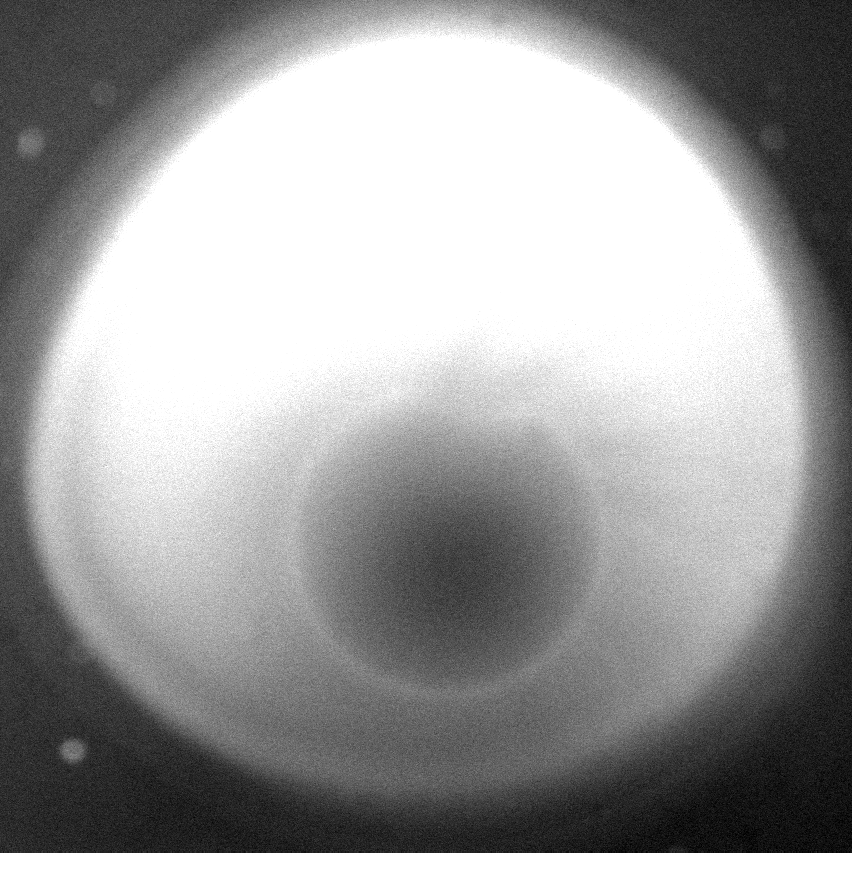
\includegraphics[width=0.3\textwidth]{figs/ch04/ring}
\label{fig:ring}
\end{SCfigure} 

The partition coefficients for NTF2-F and mCherry are shown in Fig.~\ref{fig:frac-bound} along with the corresponding fraction bound.  As expected, the partition coefficients NTF2-F and mCherry are very similar in the no-nup hydrogels, while the NTF2-F partition coefficient increases for FSFG hydrogels due to binding.  The FSFG concat-2 hydrogels show the highest NTF2-F partition coefficient, likely because there are more FG repeats in total.  The fraction bound follows similar trends, although the difference between the FSFG concat-1 and concat-2 hydrogels is less pronounced.  The fraction of NTF2-F bound to the no-nup hydrogels is indistinguishable from zero.

\begin{SCfigure}
\caption{(A) Partition coefficients for NTF2-F and mCherry in each of the three experimental conditions.  (B) Fraction of NTF2-F bound as calculated using Sec.~\ref{sec:part-coeff}.  All errors are standard error of the mean.\\}
\centering
\includegraphics[width=0.7\textwidth]{figs/ch04/fraction-bound}
\label{fig:frac-bound}
\end{SCfigure} 

Figure~\ref{fig:curves} shows normalized recovery curves for all hydrogels in the dataset.  In addition to the normalization described in Sec.~\ref{sec:photobleaching}, these curves were also scaled so that the pre-bleach average bleach spot intensity was one.  Dark curves show the average NTF2 and mCherry recovery curves for each condition.  The most obvious difference between conditions is the greater bleach depth for NTF2-F in FSFG hydrogels.  Bleach depth stays roughly constant for mCherry between conditions.

\begin{figure}
\caption{Recovery curves for (A) no-nup, (B) FSFG concat-1, and (C) FSFG concat-2 hydrogels.  All curves are shown for both NTF2-F and mCherry.  Dark lines are averaged curves.  Pre-bleach intensity set to one. \\}
\centering
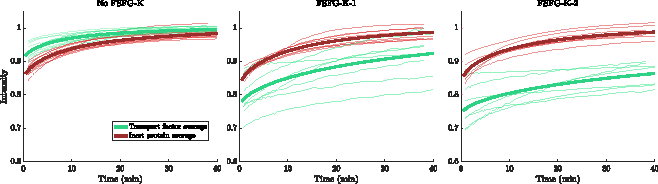
\includegraphics[width=\textwidth]{figs/ch04/curves}
\label{fig:curves}
\end{figure} 

Finally, the observed diffusion constants for NTF2-F and mCherry were calculated using the Fourier series model.  Mean values for each of the experimental conditions are shown in Fig.~\ref{fig:bound-diffusion} along with calculated bound diffusion constants.  The observed diffusion for NTF2-F and mCherry was roughly equal in the no-nup hydrogels, but NTF2-F has a much lower diffusion constant in the FSFG conditions, due to binding.  Two-tailed t-tests were conducted with the null hypothesis that $D_B = 0$.  For FSFG concat-1, the resulting p-value was $p = 0.025$; for FSFG concat-2, it was $p = 0.13$.  There is no distinguishable difference between $D_B$ for FSFG concat-1 and FSFG concat-2, which may be due to the lack of sensitivity in our measurements.

\begin{SCfigure}
\caption{(A) Observed diffusion constant for NTF2-F and mCherry in each of the three experimental conditions. (B) Calculated values of the bound diffusion constant $D_B$ for NTF2-F in the FSFG hydrogels.  All errors shown are standard error of the mean. \\}
\centering
\includegraphics[width=0.7\textwidth]{figs/ch04/bound-diffusion}
\label{fig:bound-diffusion}
\end{SCfigure} 

%% cct1 The t-value is 2.586766. The value of p is .025284. The result is significant at p < .05.
%% cct2 The t-value is 1.766134. The value of p is .127806. The result is not significant at p < .05.
%% ctrl diffusion constants green and red The t-value is 0.71937. The p-value is .477873. The result is not significant at p < .05.

%% cct1 red and green diffusion constants The t-value is -3.42286. The p-value is .002435. The result is significant at p < .05.

%% cct2 red and green diffusion constants The t-value is -4.98352. The p-value is .000096. The result is significant at p < .05.

\section{Discussion} 

Our goal was to create a material in which we could measure and test the properties of bound diffusion.  These results suggest that we can indeed measure non-zero bound diffusion, although there is no statistically significant difference between Nups of different lengths and valencies.  Smaller effects would be measurable if the fraction of transport factor bound ($p_B$) increased, as then the contribution of bound diffusion to the observed diffusion would become more prominent.  The most straightforward way of increasing the fraction bound is to increase the concentration of tethered Nups within the gel, a task which has proven difficult.  However, this dataset still provides a check on the predictions of our model.

Our bound-state diffusion model can predict the values of bound diffusion constant $D_B$ that we expect to observe, provided we input an estimate of the off-rate $\koff$ and assume that tethered diffusion the only mechanism of bound-state mobility (Appendix~\ref{appx:dataset}).  Taking $K_D \approx 0.5$ mM for FSFG concat-1 and $K_D \approx 0.4$ mM for FSFG concat-2, we can predict $D_B$ for each FSFG hydrogel \cite{hayama18}.  For FSFG concat-1 hydrogels, the predicted bound diffusion constant is $D_B = 6.9\pm0.3$ $\mu$m$^2$/s; for FSFG concat-2 gels this value is $D_B = 9.3\pm0.3$ $\mu$m$^2$/s.  These values are consistent with our measured mean values of $D_B = 5.6\pm2.3$ $\mu$m$^2$/s for FSFG concat-1 gels and $D_B = 5.2\pm3.2$ $\mu$m$^2$/s for FSFG concat-2 gels.  However, the large standard error in our measurements suggests that better measurements are needed before we can strongly state that our model has accurately predicted the bound diffusion constant.

% cct2 measured and predicted The t-value is -1.56925. The p-value is .14257. The result is not significant at p < .05.

Future work could productively focus on more precisely measuring the bound diffusion constant for transport factors interacting with Nups of various length and binding valency.  We expect that longer Nups should lead to higher bound diffusion.  If other experimental parameters such as total Nup concentration, binding affinity, and free diffusion constant can be varied in a controlled way, other predictions of the bound-diffusion model could be tested.  Additionally, other systems of transient binding could be tested using these hydrogel models to determine how universal bound diffusion is in biological systems \cite{piccolo14,olmsted01,lai09}.

The hydrogel nuclear pore mimics discussed in this chapter do not reproduce the selectivity properties of nuclear transport; the tethered Nup concentration is too low and the transport factor - Nup dissociation constant is too high.  However, they do provide a platform from which to measure bound diffusion.  Non-zero bound diffusion of transport factors was measured when Nups were tethered to the hydrogel.  This represents a first step towards understanding the effect of bound diffusion on selective biofilters.

